\chapter{Evaluation} \label{chap:Evaluation}
In dem Kapitel Evaluation sollen die Ergebnisse der angewendeten Methodik präsentiert werden. Des Weiteren wird eine Anforderungsanalyse durchgeführt, um zu beurteilen, welche Anforderungen umgesetzt wurden. Sollen einige nicht umsetzbar gewesen sein, so werden diese in diesem Abschnitt erläutert.

\section{Ergebnisevaluation der Vergleiche} \label{sec:Evaluation_Ergebnisevaluation}
In der Evaluation sollen die Ergebnisse, welche aus den Vergleichen stammten präsentiert werden. Dabei wird sich am Vorgehen orientiert.

\subsection{Evaluation der Baseline Vergleiche}
Basierend auf dem Vorgehen (siehe \ref{sec:Konzept_Vorgehen}) wird mit den Baseline Vergleichen begonnen. Bei diesen handelt es sich um die Vergleiche, welche von  nicht optimierten (baseline) Agenten durchgeführt worden sind (siehe Abbildung \ref{fig:Agenten}). Diese Agenten wurden in einem Trainingsverlauf, entsprechend der Beschreibung in Abschnitt \ref{sec:Konzept_Datenerhebung}, trainiert. 
Während dieses Prozesses wurden die Trainingsdaten erhoben, die im weiteren Verlauf graphisch dargestellt werden. Darauffolgend wurden die Testdaten in Testläufen ermittelt, welche im Folgenden tabellarisch ausgewertet werden.

\subsubsection{Performance}
Einleitend in die Baseline Vergleichsauswertung soll mit der Performance gestartet werden. Dabei ist in der Abbildung \ref{fig:Baseline_01_performance} die Performance bzw. der Apfeldurchschnitt der letzten 100 Epochs pro Epoch des ersten Baseline Vergleiches abgebildet.\\
Die DQN Agenten waren in den Vergleichen nicht in der Lage, eine durchschnittliche Apfelsammelrate von 30 Äpfeln pro Spiel zu erreichen. 
Eine vermutliche Erklärung warum die Agenten des DQN Algorithmus keine guten Leistungen erzielen konnte, liegt in der Wahl von Zufallsaktionen. Die Komplexität des Spiels Snake steigt gegen Ende immer mehr an, da die Snake, mit zunehmenden Spielfortschritt, keine nicht zielführenden Schritte mehr gehen darf. In einer beengten Spielsituation könnte jeder falsche Schritt zum Tod führen, wobei durch das zufällige Wählen von Aktionen falsche Schritte unternommen würden. Dadurch, dass das Spiel immer vorzeitig beendet würde, könnte der DQN Algorithmus auch seine Leistung nicht weiter steigern, weil ihm die Daten zum Lernen fehlten.
\begin{figure}[H]
	\centering
	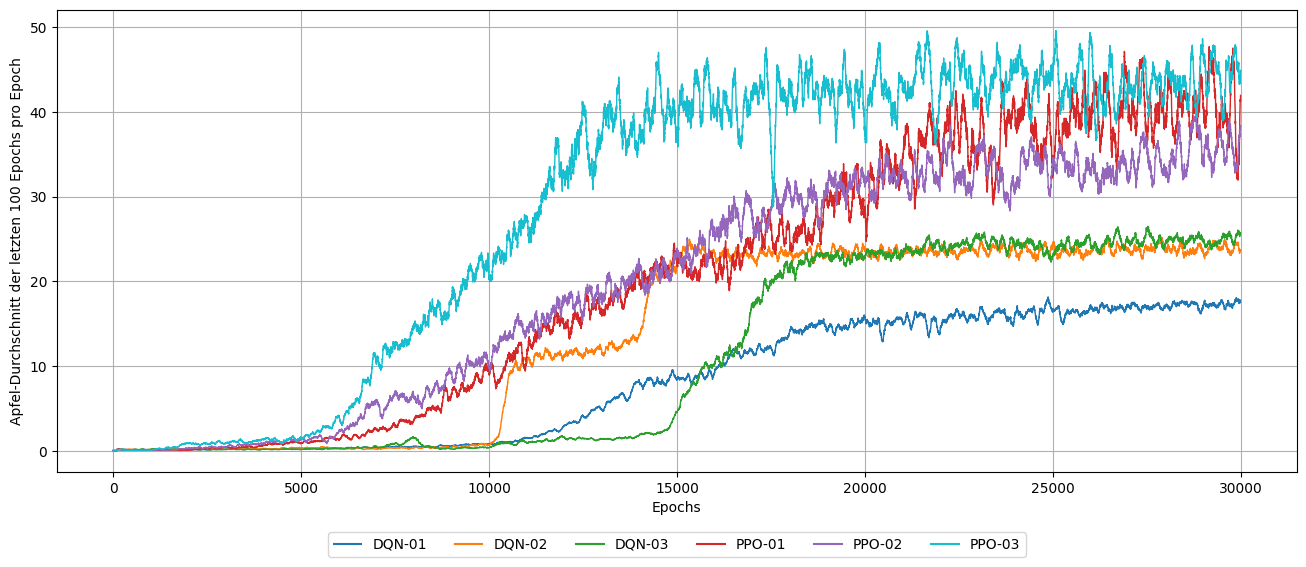
\includegraphics[scale=0.4517]{Abbildungen/Evaluation/performance-rate_baseline_01.png}
	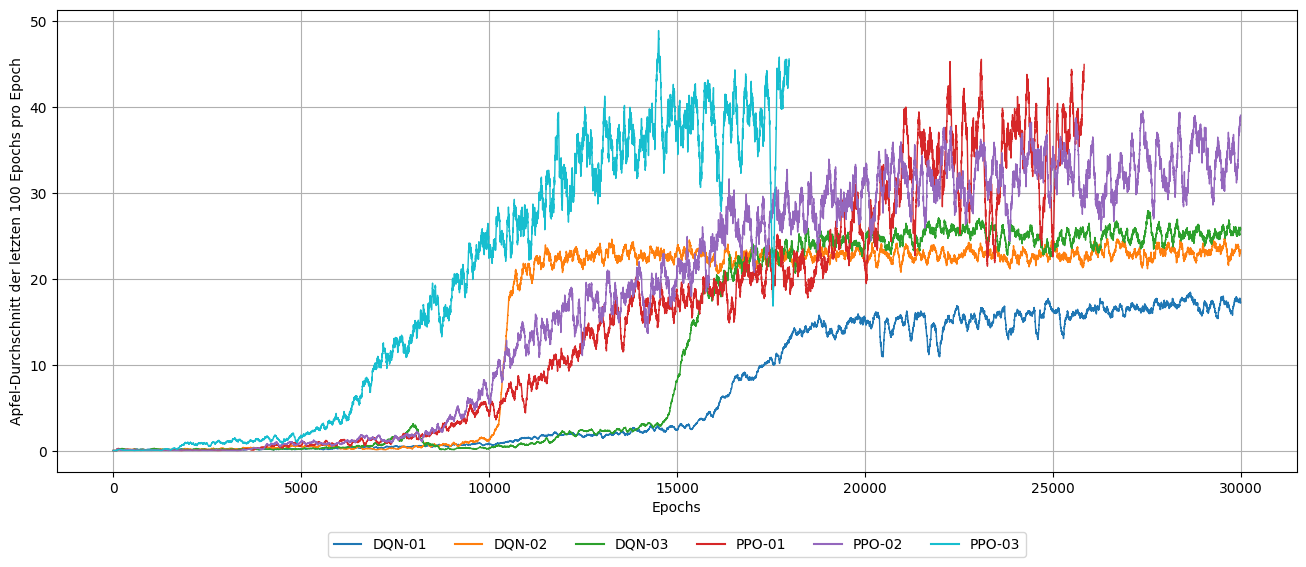
\includegraphics[scale=0.4515]{Abbildungen/Evaluation/performance-rate_baseline_02.png}
	\caption[Baseline Vergleich Performance]{Baseline Vergleich eins (oben) und zwei (unten) der Performance}
	\label{fig:Baseline_01_performance}
\end{figure}
Besonders die Leistungen der PPO Agenten PPO-03 und PPO-01 konnten, in den Vergleichen, überzeugen. Diese beiden Agenten waren ebenfalls die einzigen, welche es geschafft haben den Trainingsverlauf vorzeitig, mit einer Siegrate von 60\%, abzubrechen. 
Der PPO-03 kann dabei besonders mit seinem schnellen Lernerfolg punkten, wohingegen der PPO-01 mit seiner Stetigkeit überzeugen kann.
\begin{longtable}[h]{|p{2.7cm}|p{3cm}|p{3cm}|p{2cm}|p{2cm}|}
	\hline
	Agent & Apfel-durchschnitt-BV-1 & Apfel-durchschnitt-BV-2 & Varianz-BV-1 & Varianz-BV-2 \\
	\hline
	DQN-01 & 18.493 & 17.069 & 15.817 & 19.526 \\
	\hline
	DQN-02 & 27.876 & 24.969 & 44.968 & 30.306 \\
	\hline
	DQN-03 & 25.410 & 25.490 & 45.609 & 46.872 \\
	\hline
	PPO-01 & 49.854 & 42.201 & 614.484 & 794.192 \\
	\hline
	PPO-02 & 41.002 & 36.463 & 171.257 & 369.649 \\
	\hline
	PPO-03 & 53.975 & 49.084 & 302.203 & 565.363\\
	\hline
\caption{Testdatenauswertung der Performance}
\label{tab:Evaluation_Testdaten_Performance} 
\end{longtable}
Auch die Auswertung der Testdaten (siege Tabelle \ref{tab:Evaluation_Testdaten_Performance}) zeigt den, sich in den Trainingsdaten abzeichnenden, Trend. So erbringt der PPO-03 die beste und der PPO-01 die zweitbeste Leistung. Die Varianz der Agenten PPO-03 und PPO-01 zeigt jedoch, dass die Leistungen noch verbesserbar sind.\\
Aufgrund der erzielten Performance dieser PPO Agenten ist daher festzustellen, dass diese beiden (PPO-03 und PPO-01) das Evaluationskriterium der Performance am besten erfüllt haben. Sie sind daher die Sieger im Evaluationskriterium der Performance.

\subsubsection{Siegrate}
Ähnlich, wie mit der Performance, sieht es auch mit dem Evaluationskriterium der Siegrate aus (siehe Abbildung \ref{fig:Baseline_winrate}).\\
Die PPO Agenten PPO-03 und PPO-01 besitzen die besten Siegraten während des Trainings (siehe Abbildung \ref{fig:Baseline_winrate}). 
Die DQN Agenten sind nicht in der Lage gewesen, Siege zu erreichen und fallen daher aus der Betrachtung heraus.\\
Der PPO-02 zeigt eine geringe Siegrate, trotz ähnlicher Performances zu den Agenten PPO-01 und PPO-03 (siehe Abbildung \ref{fig:Baseline_01_performance}).
\begin{longtable}[h]{|p{3.7cm}|p{4cm}|p{4cm}|}
	\hline
	Agent & Siegraten-durchschnitt-BV-1 & Siegraten-durchschnitt-BV-2 \\
	\hline
	PPO-01 & 0.7654 & 0.626 \\
	\hline
	PPO-02 & 0.099 & 0.086  \\
	\hline
	PPO-03 & 0.668 & 0.662  \\
	\hline
	\caption{Testdatenauswertung der Baseline Siegrate}
	\label{tab:Evaluation_Testdaten_Winrate} 
\end{longtable}
Auch die Testdaten in der Tabelle \ref{tab:Evaluation_Testdaten_Winrate}, zeigt, dass die PPO Agenten PPO-01 und PPO-03 die Sieger sind, wobei dieses Mal der PPO-01 bessere Resultate in den Testdaten erzielen konnte als PPO-03. Es ist daher festzuhalten, dass der PPO-01 und PPO-03 die Sieger im Evaluationskriterium der Siegrate sind .
\begin{figure}[H]
	\centering
	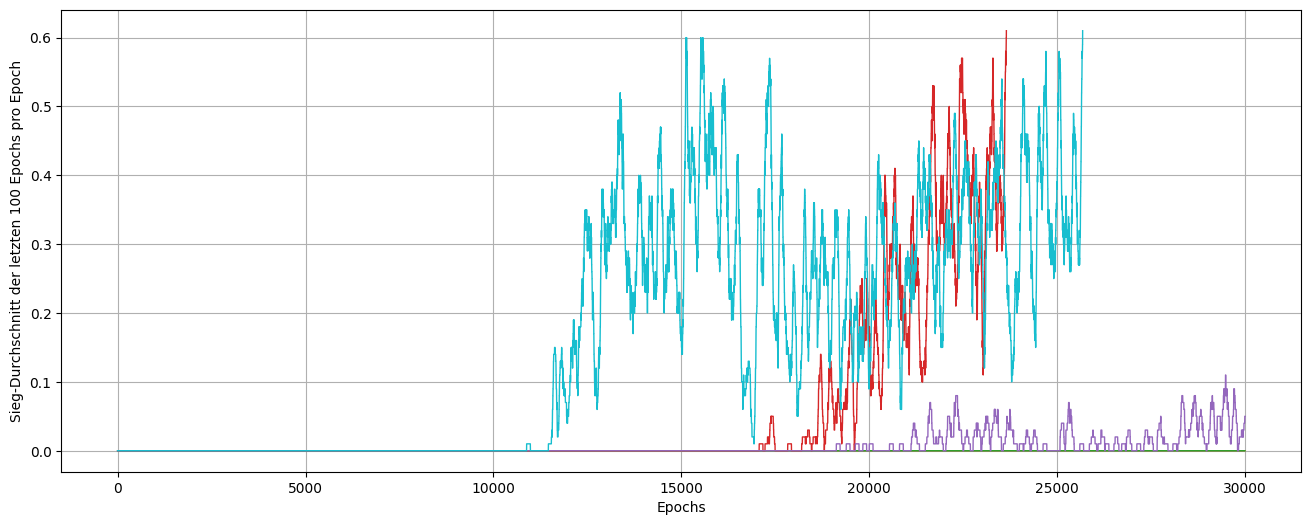
\includegraphics[scale=0.4517]{Abbildungen/Evaluation/win-rate_baseline_01.png}
	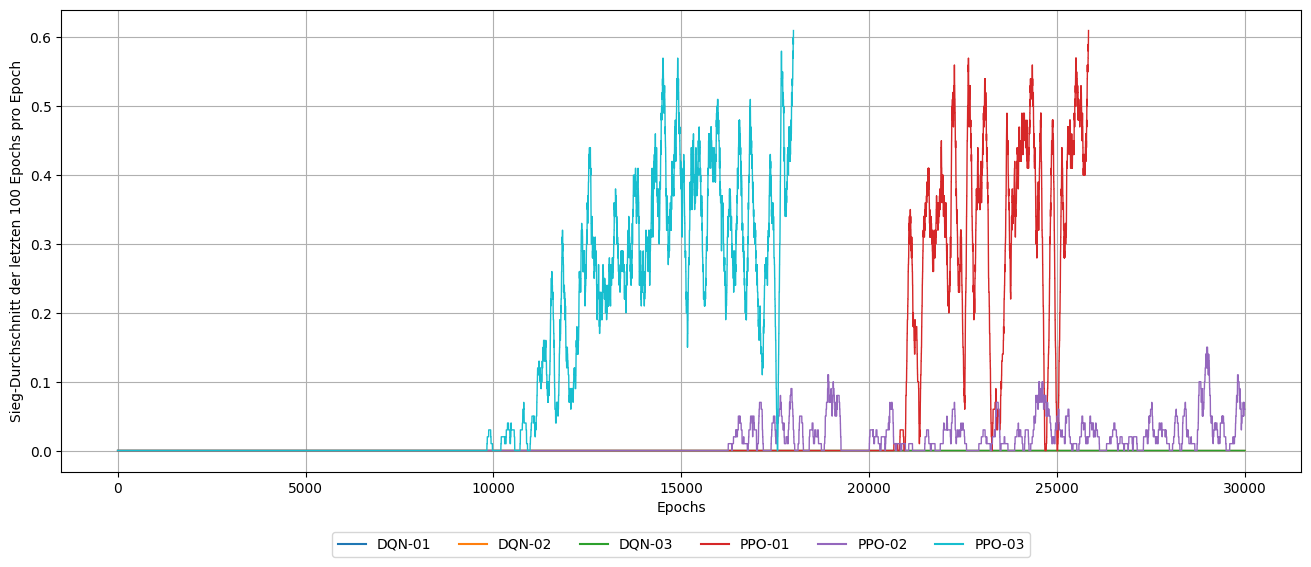
\includegraphics[scale=0.4515]{Abbildungen/Evaluation/win-rate_baseline_02.png}
	\caption[Baseline Vergleich Siegrate]{Baseline Vergleich eins (oben) und zwei (unten) der Siegrate}
	\label{fig:Baseline_winrate}
\end{figure}

\subsubsection{Effizienz}
\begin{longtable}[h]{|p{3.5cm}|p{3.0cm}|p{3.0cm}|}
	\hline
	Agent & Effizienz-durchschnitt-BV-1 & Effizienz-durchschnitt-BV-2  \\
	\hline
	DQN-01 & 0.144 & 0.154  \\
	\hline
	DQN-02 & 0.132 & 0.138  \\
	\hline
	DQN-03 & 0.129 & 0.133  \\
	\hline
	PPO-01 & 0.077 & 0.069 \\
	\hline
	PPO-02 & 0.114 & 0.090 \\
	\hline
	PPO-03 & 0.097 & 0.075 \\
	\hline
	\caption{Testdatenauswertung der Baseline Effizienz}
	\label{tab:Evaluation_Testdaten_Effizienz} 
\end{longtable}
Bei der Effizienz treten interessante Effekte auf. Wie in der Abbildung \ref{fig:Baseline_Effizienz} zu erkennen ist, sind die DQN Agenten DQN-01 und DQN-02 diejenigen, welche die beste Effizienz-Leistung erbringen. Die Effizienz ist dabei jedoch definiert als Äpfel pro Schritt. 
Die Effizienzbestimmung ist jedoch nicht abhängig von der erbrachten Performance. 
Darum bieten die Agenten DQN-01 und DQN-02 die besten Effizienzen, bei niedrigeren Performances. 
Denkbar wären diese in Einsatzgebieten mit wenigen Zielen aber großen Distanzen, sodass der Effizienzcharakter des Agenten hilft Kraftstoff oder Energie, am Beispiel der unbemannter Drohnen, zu sparen.\\
Die Tabelle \ref{tab:Evaluation_Testdaten_Effizienz} unterstützt die Trainingsergebnisse. In den Testläufen hatte der DQN-02 Agent eine, im Mittel, geringfügig bessere Effizienz als der DQN-03. Darum sind die DQN Agenten DQN-01 und DQN-02 die Siegen dieses Effizienz-Vergleiches auf reiner Basis der Effizienz.
\begin{figure}[H]
	\centering
	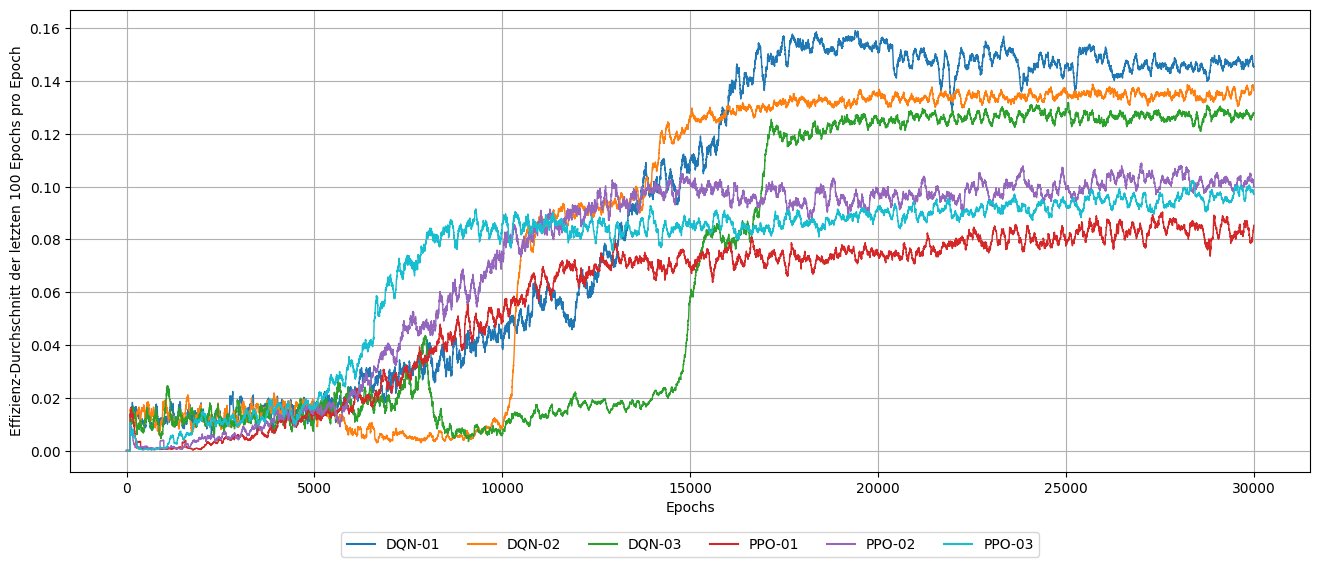
\includegraphics[scale=0.4517]{Abbildungen/Evaluation/effizienz-rate_baseline_01.png}
	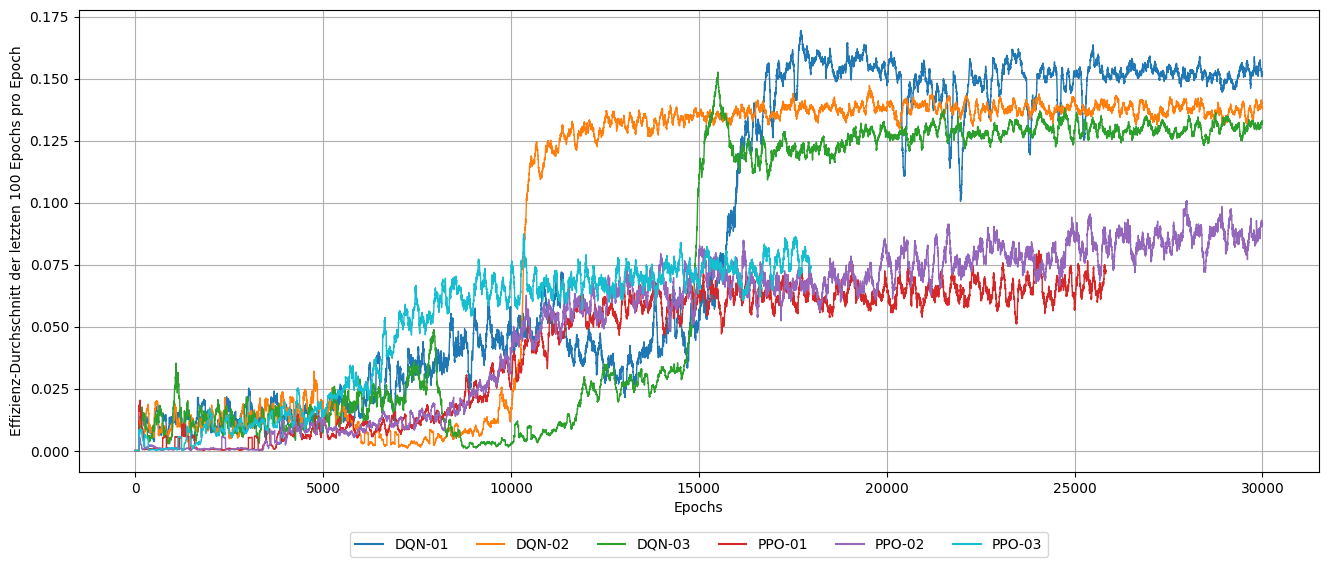
\includegraphics[scale=0.4515]{Abbildungen/Evaluation/effizienz-rate_baseline_02.png}
	\caption[Baseline Vergleich Effizienz]{Baseline Vergleich eins (oben) und zwei (unten) der Effizienz}
	\label{fig:Baseline_Effizienz}
\end{figure}

\subsubsection{Robustheit}
Die Robustheit stellt ein besonderes Evaluationskriterium dar, denn sie wird nur aus Testdaten bestimmt. Es existieren daher keine Trainingsgrafiken. Die Robustheit ist definiert als die Performance auf unbekannten Spielfeldern, mit variierenden Größen von (6x6) zu (10x10). Dabei treten alle Spielfeldgrößen gleichverteilt häufig auf.
\begin{longtable}[h]{|p{4.8cm}|p{1.5cm}|p{1.5cm}|p{1.5cm}|p{1.5cm}|p{1.5cm}|}
	\hline
	Agent / Apfeldurchschnitt auf Spielfeld mit der Größe & (6x6) & (7x7) & (8x8) & (9x9) & (10x10) \\
	\hline
	DQN-01 & 14.514 & 16.552 & 18.656 & 20.428 & 22.666 \\
	\hline
	DQN-02 & 20.177 & 24.337 & 27.986 & 31.660 & 34.304 \\
	\hline
	DQN-03 & 18.082 & 21.896 & 25.335 & 28.052 & 30.002 \\
	\hline
	PPO-01 & 25.143 & 24.081 & 50.580 & 41.568 & 41.302 \\
	\hline
	PPO-02 & 27.149 & 34.946 & 41.025 & 41.561 & 39.698 \\
	\hline
	PPO-03 & 30.217 & 36.844 & 53.107 & 53.503 & 51.559 \\
	\hline
	\caption{Testdatenauswertung der Robustheit für Baseline Vergleich 1}
	\label{tab:Evaluation_Testdaten_Robustheit_1} 
\end{longtable}
\begin{longtable}[h]{|p{4.8cm}|p{1.5cm}|p{1.5cm}|p{1.5cm}|p{1.5cm}|p{1.5cm}|}
	\hline
	Agent / Apfeldurchschnitt auf Spielfeld mit der Größe & (6x6) & (7x7) & (8x8) & (9x9) & (10x10) \\
	\hline
	DQN-01 & 13.259 & 15.291 & 17.122 & 18.734 & 20.336 \\
	\hline
	DQN-02 & 18.426 & 21.958 & 25.007 & 27.854 & 30.445 \\
	\hline
	DQN-03 & 18.595 & 22.271 & 25.245 & 27.902 & 30.244 \\
	\hline
	PPO-01 & 19.793 & 21.653 & 43.447 & 36.957 & 65.815 \\
	\hline
	PPO-02 & 22.422 & 29.334 & 37.193 & 41.107 & 41.097 \\
	\hline
	PPO-03 & 24.471 & 29.740 & 49.447 & 50.309 & 69.691 \\
	\hline
	\caption{Testdatenauswertung der Robustheit für Baseline Vergleich 2}
	\label{tab:Evaluation_Testdaten_Robustheit_2} 
\end{longtable}
Wie bei den DQN-Agenten zu beobachten ist, steigt die Anzahl der gesammelten Äpfel ungefähr linear zur nächstgrößeren Spielfeldgröße. Dies zeugt jedoch von einer schlechten Robustheit, da die Komplexität des Spiels Snake mit zunehmender Spielfeldgröße nicht linear sondern exponentiell zunimmt, aufgrund der Ausdehnung des Möglichkeitsraumes. 
Die DQN-Agenten erreichen auf kleineren Spielfeldgrößen bessere Ergebnisse als auf der Standard Spielfeldgröße von 8x8. Sollte sich jedoch das Spielfeld vergrößern, so stagnieren ihre Leistungen.
Bei den PPOs zeigt sich ein ähnliches Bild. Ihre Leistungen steigen ebenfalls nicht mit dem sich vergrößernden Spielfeld an. Jedoch waren der PPO-03 und der PPO-01 in der Lage die besten Ergebnisse in der unbekannten Gebieten zu erzielen. Im Baseline Run 2 war es dem PPO-03 sogar möglich, ein deutlich besseres Ergebnis zu erzielen, als mit der Standard Spielfeldgröße (8, 8).\\
Daher sind die Agenten PPO-03 und PPO-01 die Gewinner Agenten was das Evaluationskriterium der Robustheit betrifft.

\subsection{Evaluation der Optimized Vergleiche}
Nach der Durchführung der Baseline Vergleiche werden nun, entsprechend des Vorgehens (siehe \ref{sec:Konzept_Vorgehen}), die Baseline Gewinner Agenten (siehe Abbildung \ref{fig:Vorgehen}) optimiert und dann untereinander verglichen. Dabei werden ebenfalls die Baseline Agenten Gewinner mit in den Vergleich eingebunden. Die Ergebnisse dieser Vergleiche finden sich in den Folgenden Abschnitten.

\subsubsection{Performance}
\begin{figure}[H]
	\centering
	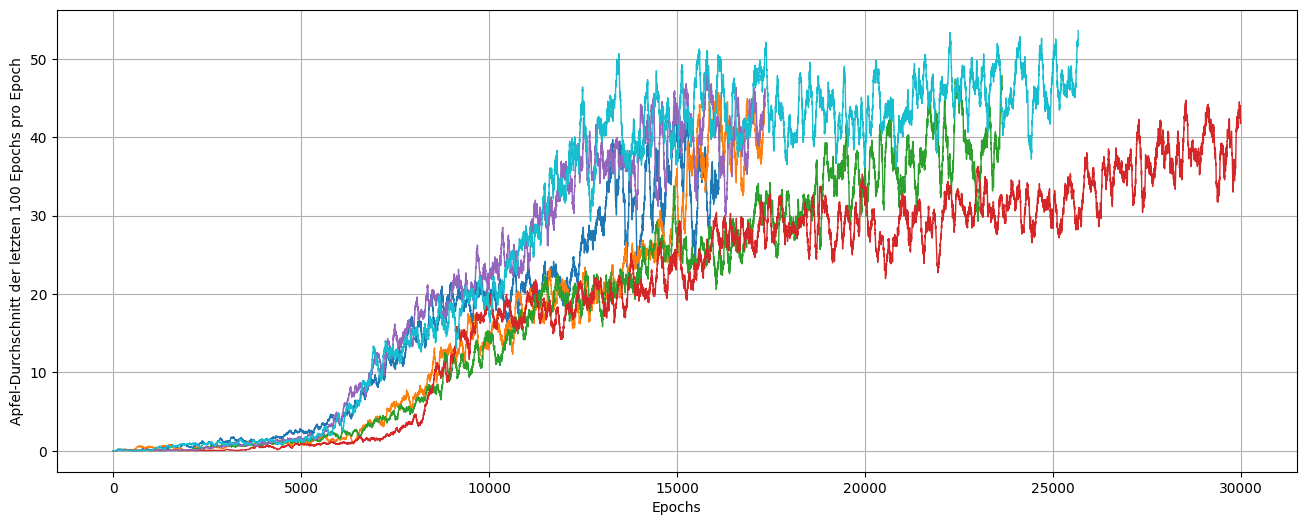
\includegraphics[scale=0.4517]{Abbildungen/Evaluation/performance-rate_optimized_01.png}
	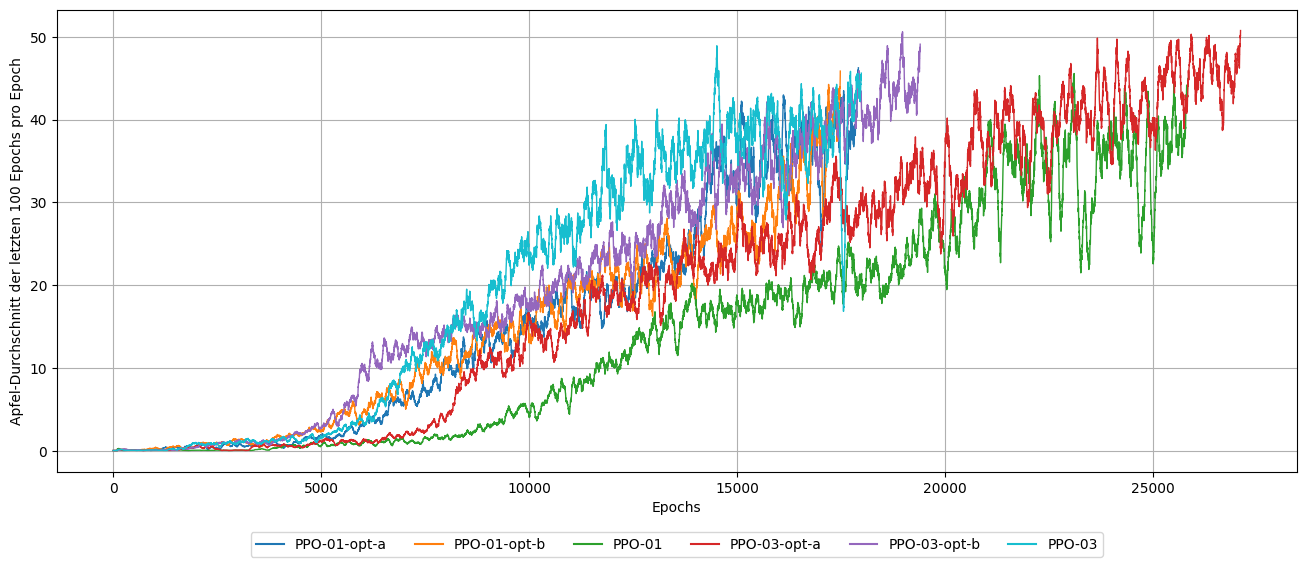
\includegraphics[scale=0.4515]{Abbildungen/Evaluation/performance-rate_optimized_02.png}
	\caption[Optimized Vergleich Performance]{Baseline Vergleich eins (oben) und zwei (unten) der Effizienz}
	\label{fig:Optimized_Performance}
\end{figure}
Wie in Abbildung \ref{fig:Optimized_Performance} zu erkennen ist, konnten alle Agenten, mit Ausnahme vom PPO-03-opt-a im OV-1 (Optimized Vergleich 1), den Lernprozess vorzeitig beenden. Auffällig ist, dass die Agenten PPO-01-opt-a (dunkelblau), PPO-01-opt-b (orange) und der PPO-03-opt-b (lila) Agent  ungefähr zeitgleich eine Siegrate von 60\% erreichten, gefolgt vom den Baseline Agenten und PPO-03-opt-a.
\begin{longtable}[h]{|p{2.7cm}|p{3cm}|p{3cm}|p{2cm}|p{2cm}|}
	\hline
	Agent & Apfel-durchschnitt-BV-1 & Apfel-durchschnitt-BV-2 & Varianz-BV-1 & Varianz-BV-2 \\
	\hline
	PPO-01 & 49.854 & 42.201 & 614.484 & 794.192 \\
	\hline
	PPO-03 & 53.975 & 49.084 & 302.203 & 565.363 \\
	\hline
	PPO-01-opt-a & 45.071 & 42.227 & 746.026 & 748.823 \\
	\hline
	PPO-01-opt-b & 47.745 & 47.907 & 687.583 & 680.407 \\
	\hline
	PPO-03-opt-a & 46.438 & 54.444 & 551.219 & 303.706 \\
	\hline
	PPO-03-opt-b & 49.630 & 50.581 & 607.097 & 530.553 \\
	\hline
	\caption{Testdatenauswertung der Performance}
	\label{tab:Evaluation_Testdaten_Performance_Optimized} 
\end{longtable}
Aus den Testdaten (siehe Tabelle \ref{tab:Evaluation_Testdaten_Performance_Optimized}) geht hervor, dass sowohl PPO-03 als auch PPO-03-opt-a die besten Agenten dieses Vergleiches sind. Jedoch konnte der Baseline Agent PPO-03 die besseren Ergebnisse, im Mittel, vorweisen. Mit einer durchschnittlichen Performance von 51.5295 Äpfeln in den Testläufen, stellt der PPO-03 den optimalen Agenten für das Evaluationskriterium der Performance dar. Jedoch verrät die Varianz ein instabiles Sammelverhalten, sodass bei der Anwendung dieses Agenten davon auszugehen ist, dass dieser die gezeigte Leistung nicht konstant erbringen wird.

\subsubsection{Siegrate}
\begin{longtable}[h]{|p{3.7cm}|p{4cm}|p{4cm}|}
	\hline
	Agent & Siegraten-durchschnitt-BV-1 & Siegraten-durchschnitt-BV-2 \\
	\hline
	PPO-01 & 0,765 & 0,626 \\
	\hline
	PPO-03 & 0,668 & 0,662  \\
	\hline
	PPO-01-opt-a & 0,681 & 0,611  \\
	\hline
	PPO-01-opt-b & 0,732 & 0,733 \\
	\hline
	PPO-03-opt-a & 0,478 & 0,721 \\
	\hline
	PPO-03-opt-b & 0,741 & 0,727 \\
	\hline
	\caption{Testdatenauswertung der Optimized Siegraten}
	\label{tab:Evaluation_Testdaten_Winrate_Optimized} 
\end{longtable}
Bei der Siegrate konnten fast immer alle Agenten sehr guten Ergebnissen erzielen. Einzig PPO-03-opt-a lag im ersten Optimized Vergleich unter der erwarteten Siegrate von 60\%, wie in Abbildung \ref{fig:Optimized_Winrate} zu erkennen ist.\\
\\Wie die Auswertung der Testdaten (siehe Tabelle \ref{tab:Evaluation_Testdaten_Winrate_Optimized}) aufzeigt, liefern die Agenten PPO-01-opt-b und PPO-03-opt-b sehr gute Ergebnisse. Jedoch gewinnt der PPO-03-opt-b diesen Vergleich mit einer durchschnittlichen Siegrate von 0,73405, dicht gefolgt vom PPO-01-opt-b mit 0,7325. Insgesamt ist dennoch zu bemerken, dass dieser kleine Abstand in der Siegrate auch durch Zufallseffekte zu erklären ist.
\begin{figure}[H]
	\centering
	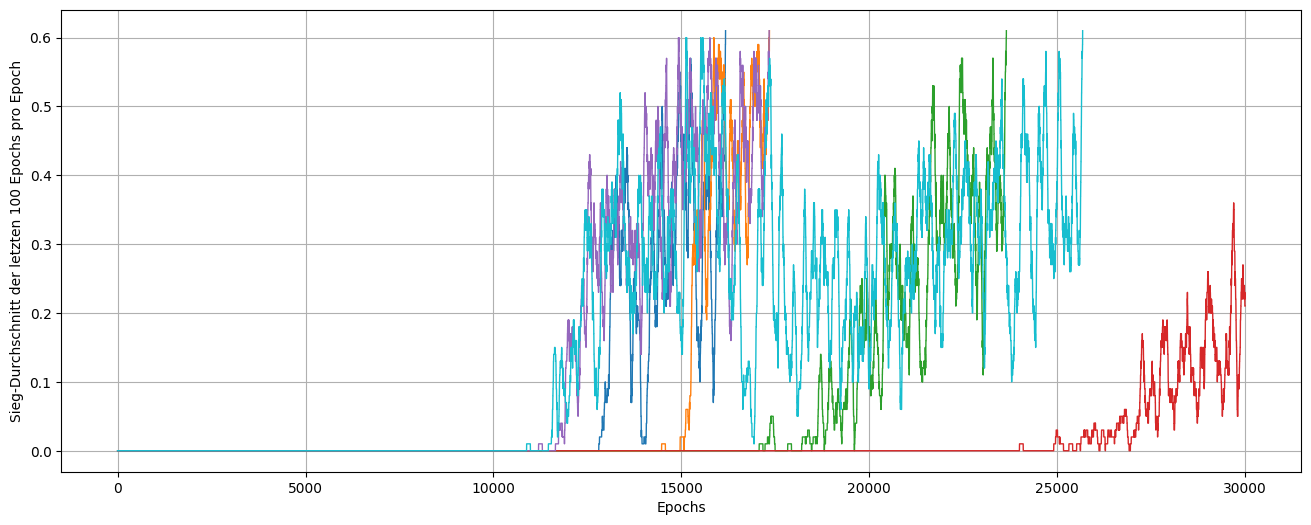
\includegraphics[scale=0.4517]{Abbildungen/Evaluation/win-rate_optimized_01.png}
	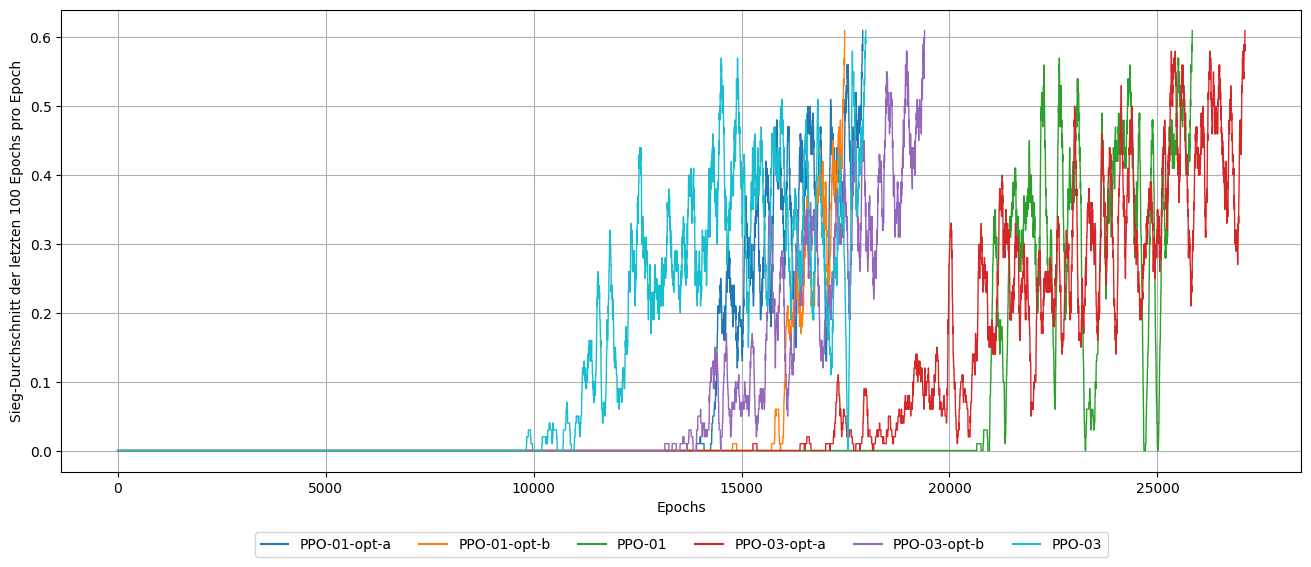
\includegraphics[scale=0.4515]{Abbildungen/Evaluation/win-rate_optimized_02.png}
	\caption[Optimized Vergleich Siegrate]{Optimized Vergleich eins (oben) und zwei (unten) der Siegrate}
	\label{fig:Optimized_Winrate}
\end{figure}

\subsubsection{Effizienz}
folgt im selben Stil.

\subsubsection{Robustheit}
Nach den Testauswertungen (siehe Tabelle \ref{tab:Evaluation_Testdaten_Robustheit_1_Optimized} und \ref{tab:Evaluation_Testdaten_Robustheit_2_Optimized}) hat sich der PPO-01-opt-b als der robusteste Agent dargestellt. Von allen Agenten weist er die kontinuierlichste Performance vor. Besonders auf größeren Spielfeldern zeigt er eine gute Leistung und damit eine solide Robustheit.\\
Es ist daher festzuhalten, dass der PPO-01-opt-b der Sieger der Vergleiches für das Evaluationskriterium der Robustheit ist.
\begin{longtable}[h]{|p{4.8cm}|p{1.5cm}|p{1.5cm}|p{1.5cm}|p{1.5cm}|p{1.5cm}|}
	\hline
	Agent / Apfeldurchschnitt auf Spielfeld mit der Größe & (6x6) & (7x7) & (8x8) & (9x9) & (10x10) \\
		\hline
	PPO-01 & 25.143 & 24.081 & 50.580 & 41.568 & 41.302 \\
	\hline
	PPO-03 & 30.217 & 36.844 & 53.107 & 53.503 & 51.559 \\
	\hline
	PPO-01-rgs-opt-a & 20.823 & 23.032 & 44.746 & 39.912 & 45.084 \\
	\hline
	PPO-01-rgs-opt-b & 26.135 & 31.067 & 52.574 & 56.541 & 80.265 \\
	\hline
	PPO-03-rgs-opt-a & 25.218 & 34.149 & 47.113 & 51.403 & 56.545 \\
	\hline
	PPO-03-rgs-opt-b & 24.966 & 30.395 & 47.946 & 57.580 & 74.758 \\
	\hline
	\caption{Testdatenauswertung der Robustheit für Optimized Vergleich 1}
	\label{tab:Evaluation_Testdaten_Robustheit_1_Optimized} 
\end{longtable}
\begin{longtable}[h]{|p{4.8cm}|p{1.5cm}|p{1.5cm}|p{1.5cm}|p{1.5cm}|p{1.5cm}|}
	\hline
	Agent / Apfeldurchschnitt auf Spielfeld mit der Größe & (6x6) & (7x7) & (8x8) & (9x9) & (10x10) \\
	\hline
	PPO-01 & 19.793 & 21.653 & 43.447 & 36.957 & 65.815 \\
	\hline
	PPO-03 & 24.471 & 29.740 & 49.447 & 50.309 & 69.691 \\
	\hline
	PPO-01-rgs-opt-a & 22.534 & 24.358 & 42.942 & 42.223 & 39.528 \\
	\hline
	PPO-01-rgs-opt-b & 23.666 & 26.969 & 47.885 & 40.227 & 77.224 \\
	\hline
	PPO-03-rgs-opt-a & 29.808 & 35.390 & 54.276 & 51.236 & 59.522 \\
	\hline
	PPO-03-rgs-opt-b & 25.422 & 32.201 & 52.448 & 46.262 & 47.342 \\
	\hline
	\caption{Testdatenauswertung der Robustheit für Optimized Vergleich 2}
	\label{tab:Evaluation_Testdaten_Robustheit_2_Optimized} 
\end{longtable}

\section{Anforderungsevaluation}
Zu Beginn sollen die Anforderungen an das Environment evaluiert werden. Danach folgen die Evaluationen der Anforderungen Agenten und der Datenerhebung. Zum Schluss sollen evaluiert werden, ob alle Anforderungen bezüglich der Statistiken und der Evaluation selbst erfüllt worden sind.

\subsection{Anforderungsevaluation der Environment}
Die Hauptanforderung an das Env besagt, dass das Spiel Snake implementiert werden soll. Im Rahmen dieser Ausarbeitung wurde das Spiel Snake nach der Beschreibung in \ref{sec:Snake} implementiert. Diese Anforderung kann daher als erfüllt angesehen werden. Eine Darstellung der Implementierung findet sich im Abschnitt des Konzepts (siehe \ref{sec:Konzept_Environment}) und in der Implementierung (siehe \ref{sec:Implementierung_Environment}).\\
\\ Ebenfalls wurde die Anforderung der Standardisierten Schnittstelle (siehe \ref{sec:Anforderungen_Schnittstelle}), welche zu einer Normung und damit zu einer einfacheren Benutzung des Environment führen soll, erfüllt. Wie in den Abschnitten \ref{sec:Konzept_Schnittstelle} und \ref{sec:Implementierung_train_Methode} zu sehen ist, werden Aktionen, durch die step Methoden entgegengenommen, Rewards und Observationen zurückgegeben. Neben der step Methode wird die Observation auch noch durch die Schnittstellenmethode reset geliefert. Diese beiden Methoden spannen die standardisierte Schnittstelle auf.\\
\\ Auch sind die funktionalen Anforderungen, welche den geregelten Ablauf im Environment garantieren, beachtet worden.
So wird die Aktionsausführung (siehe \ref{sec:Anforderungen_Aktionsausführung}) durch die action Methode in der SnakeGame Klasse durchgeführt, welche von der Schnittstellenmethode step aufgerufen wird. Die reset und render Anforderungen (siehe \ref{sec:Anforderung_Reset} und \ref{sec:visualisierung_Env}) werden durch die gleichnamigen Schnittstellenmethode abgedeckt (siehe \ref{sec:Konzept_Spielablauf} und \ref{sec:Implementierung_Environment}).

\subsection{Anforderungsevaluation der Agenten}
Der nächste großer Anforderungsbereich behandelt die Agenten. Diese sollen funktionalen Anforderungen entsprechen, damit sie funktionsfähig und genormt sind. Zu diesem Zweck wurden die Anforderungen der Aktionsbestimmung und des Lernens aufgestellt. Diese stellen die grundlegenden Funktionen der Agenten dar. 
Wie im Konzept dargestellt ist, wurde sowohl der DQN als auch der PPO Agent mit einer Aktionsauswahlmethode (siehe \ref{Implementierung_act_PPO} und \ref{sec:Implementierung_act_DQN}) und einer learn Methode (siehe \ref{sec:Implementierung_learn_DQN} und \ref{sec:Implementierung_learn_PPO}) ausgestattet. Diese implementieren das geforderte Verhalten aus den Anforderungen (siehe \ref{sec:Agent_Funktionalitäten}).\\
\\Neben den funktionalen, existieren noch zwei weitere Anforderungen. Zu diesen gehört die Diversität der Algorithmen (siehe \ref{sec:Anforderungen_Diversität}).\\
Diese fordert den Vergleich verschiedener Algorithmen und dabei insbesondere des PPO und DQN Algorithmus. Mit dieser Forderung kann die entwickelte Methodik (siehe \ref{sec:Konzept_Vorgehen}) besser bewertet werden. Diese Anforderung kann ebenfalls als erfüllt angesehen werden, da sowohl ein DQN (siehe \ref{sec:Implementierung_DQN_Agent}) als auch ein PPO Agent (siehe \ref{sec:Implementierung_PPO_Agent}) implementiert wurden.\\
\\ Die andere der zwei erwähnten Anforderungen behandelt die Parametrisierung der Agenten. Das System soll mehrere Agenten gleichen Algorithmus erstellen können, welche sich jedoch durch die Hyperparameter unterscheiden sollen. Wie auch in der Evaluation der Ergebnisse (siehe \ref{sec:Evaluation_Ergebnisevaluation}) und in dem Konzept (siehe \ref{sec:Konzept_Vorstellung_Agenten})zur erkennen ist, werden mehrere Agenten des gleichen Algorithmus miteinander verglichen.

\subsection{Anforderungsevaluation an die Datenerhebung} \label{sec:Evaluation_Datenerhebung}
Auch an die Datenerhebung wurden einige Anforderungen im Rahmen dieser Ausarbeitung gestellt. Zu diesen gehört die Forderung, dass die zu erhebenden Daten mehrfach erhoben werden sollen 
(siehe \ref{sec:Anforderungen_mehrfache_Datenerhebung}). Dies soll die Validität der statistischen Untersuchung steigern. Wie im Abschnitt der Datenerhebung (siehe \ref{sec:Konzept_Datenerhebung}) und in der Evaluation der Ergebnisse zu sehen ist, werden die auszuwertenden Daten doppelt erhoben. Daher sind aus immer zwei Statistiken zu einem Evaluationskriterium zu sehen.\\
Daraus lässt sich ebenfalls schließen, dass die Daten für die Statistiken gespeichert werden. Damit wird die Anforderung der Datenspeicherung erfüllt (siehe \ref{sec:Anforderungen_Datenspeicherung}). Dies wurde darüber hinaus in dem Abschnitt der Datenerhebung des Konzepts (siehe \ref{sec:Konzept_Datenerhebung}) und in der Implementierung (siehe \ref{sec:Implementierung_train_Methode}) dargestellt.

\subsection{Anforderungen an die Statistiken}
Insgesamt sind die Anforderungen zu den Statistiken (siehe \ref{sec:Anforderungen_Statistik}) darauf ausgelegt, dass mit dem implementierten System Statistiken entsprechend der Evaluationskriterien generiert werden können. Ein solche Funktionalität wurde implementiert, wie die Abschnitte \ref{sec:Konzept_Datenerhebung_Verarbeitung} und \ref{sec:Implementierung_Statistiken} beweisen. Auch die Grafiken in der Evaluation der Ergebnisse (siehe \ref{sec:Evaluation_Ergebnisevaluation}) bestätigen dies.

\subsection{Anforderungen an die Evaluation}
In den Anforderungen der Evaluation war gefordert, das die Evaluationskriterien Performance, Effizienz Robustheit und Siegrate untersucht werden. Wie im Abschnitt Ergebnisevaluation der Vergleiche \ref{sec:Evaluation_Ergebnisevaluation} zu erkennen ist, wurde genau dies durchgeführt. Mithilfe dieser Evaluationskriterien konnte, auf Grundlage der erhobenen Statistiken, ein optimaler Agent für jedes Kriterium ausgewählt werden.